\section{本章小结}
\label{sec:kkt-summary}

本章回答的问题是：给定一个候选点，怎样只用它附近的信息判断它是否最优。答案不是一个公式，而是按顺序做的几项检查，每一项给出的结论强弱不同，见图~\ref{fig:kkt-decision-flow}。

\begin{BookInlineFigure}
  \centering
  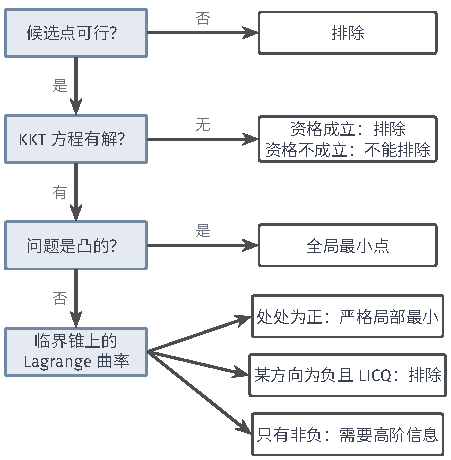
\includegraphics[width=76.3mm]{figures/05-optimization/06-constrained-optimization/tikz/kkt-decision-flow/figure.pdf}
  \caption{判断候选点的流程。左列依次是可行性、KKT方程、凸性和临界锥上的曲率四项检查，右列是对应的结论。“资格”指候选点满足的约束资格，如LICQ或MFCQ。}
  \label{fig:kkt-decision-flow}
\end{BookInlineFigure}

第一项检查是可行性，并找出活动约束。不活动的约束在局部不起作用，所以后面的条件只看活动约束和等式约束。

第二项检查是真实的局部方向。切锥只依赖可行集，它给出最根本的必要条件：局部最小点处，切锥中没有一阶下降方向。线性化锥好算，但可能多出虚假方向。LICQ和MFCQ保证两者相等，这两个条件只涉及约束函数在该点的梯度，与目标的凸性无关，并且会随约束的写法改变。

第三项检查是KKT条件。Farkas引理把“线性化锥中没有下降方向”换成负梯度属于活动梯度的非负锥，由此得到驻定、原始可行、乘子非负和互补松弛四组条件。在MFCQ下它们是局部最小点的必要条件，LICQ进一步保证乘子唯一。没有约束资格时，最小点可以没有乘子。

局部结论和全局结论要分开。目标和不等式约束函数凸、等式约束仿射时，任何KKT点都是全局最小点，这不需要约束资格。一般非凸问题中，KKT点只是候选，全局结论要靠存在性和枚举等其他依据。

第四项检查是曲率。只有一阶变化为零的方向才需要二阶判断，这些方向组成临界锥，零乘子的活动约束在其中保留单侧限制。约束的弯曲通过乘子进入Lagrange函数的Hessian，所以检查的是Lagrange Hessian在临界锥上的二次型，不是目标Hessian，也不是全空间的正定性。LICQ下二次型非负是必要条件；在某组KKT乘子下对非零临界方向严格为正是充分条件，并且给出局部二次增长，这一方向不需要约束资格。两者之间的退化情形，二阶信息判断不了。

这些条件都在已知候选点时做判断，没有回答候选点从哪里来。下一章用乘子构造整个问题的下界，把这里局部的条件变成可以检验的全局证书。可行迭代、乘子更新和局部子问题怎样产生满足这些条件的点，由第~\ref{chap:feasible-iterations}章至第~\ref{chap:nonlinear-interior-point}章研究。
